\documentclass[border=1mm]{standalone}
\usepackage{tikz}
\usepackage{amsmath}
\usetikzlibrary{shapes.geometric}
\usetikzlibrary{positioning}
\usetikzlibrary{calc, shapes.arrows}
\usetikzlibrary{backgrounds,trees,hobby}
\begin{document}
\def\connect#1#2#3{%
    % #1: starting node
    % #2: ending node
    % #3: attributes for the shape connecting nodes
    \path let
      \p1 = ($(#2)-(#1)$),
      \n1 = {veclen(\p1)},
      \n2 = {atan2(\y1,\x1)} % <- Update
    in
      (#1) -- (#2) node[#3, midway, rotate = \n2, shading angle = \n2+90, minimum        width=\n1, minimum height=1pt, inner sep=1pt] {};
}
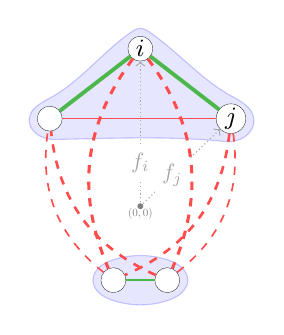
\begin{tikzpicture}
\definecolor{scattercolor1}{HTML}{800080}
\definecolor{scattercolor2}{HTML}{DD0000}
\definecolor{scattercolor3}{HTML}{009900}
\definecolor{scattercolor4}{HTML}{808000}
\definecolor{scattercolor5}{HTML}{D30E78}
\definecolor{scattercolor6}{HTML}{036ffc}
\definecolor{scattercolor7}{HTML}{eb9800}
\tikzstyle{cut-edge}=[gray!70, dashed]
\tikzstyle{vector-arrow}=[gray!70, densely dotted]
\tikzstyle{att-edge}=[scattercolor3!70]
\tikzstyle{rep-edge}=[red!70]
\tikzstyle{vertex}=[circle, draw, ultra thin, fill=white, inner sep=0.7pt, minimum width=9pt]
\tikzstyle{vector}=[rectangle, draw,inner sep=1pt,outer sep=0pt,
minimum height=5mm, minimum width=2mm, ultra thin]
% \foreach \N in {1,...,5}
%   \node[draw=none] (P\N) at ({360/5*(\N-1)+90}:1.2cm) {};

\node[vertex] (Pi) at ({90}:2.0cm) {\small{$i$}};
\node[vertex] (Pj) at ({44}:1.6cm) {\small{$j$}};
\node[vertex] (Pk) at ({290}:1.cm) {};
\node[vertex] (Pl) at ({250}:1.cm) {};
\node[vertex] (Pm) at ({136}:1.6cm) {};

\draw[->, style=vector-arrow] (0,0) -- (Pi) node [pos=0.3,fill=white,scale=0.8] {{$f_i$}};
\draw[->, style=vector-arrow] (0,0) -- (Pj) node [pos=0.4,fill=white,scale=0.8] {{$f_j$}};
% \draw[->, style=vector-arrow] (0,0) -- (Pk) node [midway,fill=white,scale=0.8] {{$f_k$}};
% \draw[->, style=vector-arrow] (0,0) -- (Pl) node [midway,fill=white,scale=0.8] {{$f_l$}};
% \draw[->, style=vector-arrow] (0,0) -- (Pm) node [midway,fill=white,scale=0.8] {{$f_m$}};

% \draw[style=att-edge] (Pi) -- (Pj) node [pos=1.2,fill=none,scale=0.7, above=0.5cm] {\textcolor{gray}{$c_{ij} = \langle f_i, f_j \rangle$}};
\draw[fill=gray, gray] (0,0) circle (.2ex);
\node[draw=none, gray, scale=0.4] (origin) at (-0.0, -0.1) {$(0, 0)$};
\draw[style=att-edge, line width = 1.4pt] (Pi) -- (Pj);
\draw[style=rep-edge, line width = 1.1pt, dashed] (Pi) to [bend left=30] (Pk);
\draw[style=rep-edge, line width = 1.1pt, dashed] (Pi) to [bend right=30] (Pl);
\draw[style=att-edge, line width = 1.4pt] (Pi) -- (Pm);
\draw[style=rep-edge, line width = 0.6pt, dashed] (Pj) to [bend left=30] (Pk);
\draw[style=rep-edge, line width = 0.95pt, dashed] (Pj) to [bend left=30] (Pl); 
\draw[style=rep-edge, line width = 0.2pt] (Pj) -- (Pm); 
\draw[style=att-edge, line width = 0.6pt] (Pk) -- (Pl); 
\draw[style=rep-edge, line width = 0.95pt, dashed] (Pk) to [bend left=30] (Pm); 
\draw[style=rep-edge, line width = 0.6pt, dashed] (Pl) to [bend left=30] (Pm); 

\begin{pgfonlayer}{background}

\draw[fill=blue!50,opacity=0.2,draw=blue]([yshift=0.1cm] Pi.north) to[closed,curve through={([yshift=0.1cm]Pi.north east) .. ([yshift=0.1cm]Pj.north) .. ([xshift=0.1cm]Pj.east) .. ([yshift=-0.1cm]Pj.south) .. ([yshift=-0.15cm]Pj.south west) .. ([yshift=-0.15cm]Pm.south east) .. ([yshift=-0.1cm]Pm.south) .. ([xshift=-0.1cm]Pm.west) .. ([yshift=0.1cm]Pm.north) .. ([yshift=0.1cm]Pi.north west)}]([yshift=0.1cm] Pi.north);

\draw[fill=blue!50,opacity=0.2,draw=blue]([yshift=0.1cm] Pk.north) to[closed,curve through={([yshift=0.1cm]Pl.north) .. ([xshift=-0.1cm]Pl.west) ([yshift=-0.1cm] Pl.south) .. ([yshift=-0.1cm]Pk.south)}]([xshift=0.1cm] Pk.east);

\end{pgfonlayer}
% \draw[style=att-edge] (Pi) -- (Pj) node [midway,fill=white,scale=0.8] {{$1.0$}};
% \draw[style=rep-edge] (Pi) -- (Pk) node [midway,fill=white,scale=0.8] {{$-1.7$}};
% \draw[style=rep-edge] (Pi) -- (Pl) node [midway,fill=white,scale=0.8] {{$-2.4$}};
% \draw[style=att-edge] (Pi) -- (Pm) node [midway,fill=white,scale=0.8] {{$1.0$}};
% \draw[style=att-edge] (Pj) -- (Pk) node [midway,fill=white,scale=0.8] {{$2.5$}};
% \draw[style=rep-edge] (Pj) -- (Pl) node [midway,fill=white,scale=0.8] {{$-1.6$}};
% \draw[style=att-edge] (Pj) -- (Pm) node [midway,fill=white,scale=0.8] {{$-1.5$}};

\end{tikzpicture}
\end{document}